%  !TeX  root  =  user_guide.tex

\section{Extension d'Édition offline}\label{sec:offlinedit}

% when the revision of a section has been finalized, 
% comment out the following line:
% \updatedisclaimer

Pour les collectes de données, il est commun d'aller sur le terrain avec un ordinateur ou 
un téléphone portable. De retour sur le réseau, les modifications doivent être 
synchronisées avec la source de données initiale, par exemple une base de données PostGIS. 
Si plusieurs personnes travaillent ensembles sur les mêmes jeux de données, il est difficile 
de fusionner les éditions à la main, même si les utilisateurs ne changent pas les mêmes 
entités.

L'extension \toolbtntwo{offline_editing_copy}{Édition offline} automatise la synchronisation 
en copiant le contenu d'une source de données (habituellement PostGIS or WFS-T) vers une 
base spatialite et en stockant les éditions offline dans des tables dédiées. Après s'être 
connecté de nouveau au réseau, il est possbile d'appliquer les éditions offline aux jeux de 
données sources.

\minisec{Utiliser l'extension}

\begin{itemize}
\item Ouvrez des couches vecteurs, par exemple d'une source de données PostGIS ou WFS-T
\item Sauvez les dans un projet
\item Pressez le bouton 'Convertir en projet offline' et sélectionnez les couches à 
sauver. Le contenu des couches est sauvé dans des tables spatialite. 
\item Éditez les couches offline.
\item Après vous être connecté au réseau de nouveau, uploadez les modifications 
avec le bouton 'Synchroniser'.
\end{itemize}

\begin{figure}[ht]
   \centering
   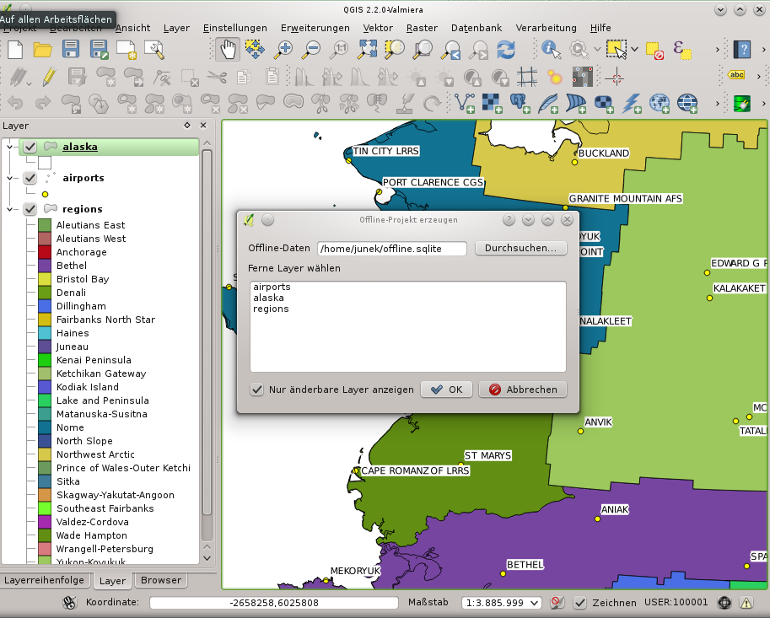
\includegraphics[clip=true, width=12cm]{create_offline_project}   
   \caption{Créer un project offline à partir des couches PostGIS ou WFS \nixcaption}
   \label{fig:offlineproject}
\end{figure}

\FloatBarrier
